\section{Background and Motivation}
\label{sec:backgroundAndMotivation}

% We review briefly the classic graph reachability formulation for a field sensitive and context sensitive pointer analysis and list three typical error situations caused by its incomplete handling of on-fly call-graph building.

% We first review two classic formulations for callsite-sensitive and field sensitive pointer analysis. Next, we motivate this work by pointing out three limitations of the traditional CFL-reachability formulation due to a lack of a built-in callgraph construction mechanism.

This paper focuses on \kcs{k} for object-oriented languages such as Java. For
a Java program, its call graph is constructed by discovering
the target methods invoked at  its virtual
callsites. For \kcs{k},
we first review 
its Andersen-style inclusion-based formulation and  its
 traditional CFL-reachability formulation \manuLFC
(\Cref{subsec:background}).
We then motivate this research with an example, by illustrating how these two
formulations handle call graph
construction, examining the limitations of \manuLFC, and finally, 
highlighting the necessity of and challenges faced in designing \LFCR, a
new CFL-reachability formulation that includes on-the-fly call graph construction
as a built-in mechanism (\Cref{subsec:motivation}). 




\begin{table}[htbp]
\begin{center}
% \vspace*{-1ex}
\begin{adjustbox}{width=1\linewidth}
\setlength{\tabcolsep}{4ex}
\def\arraystretch{1.2}
%\footnotesize
\begin{tabular}{c l@{\hspace{2.5cm}} c l }
\toprule
\textbf{Kind} & \textbf{Statement} & \textbf{Kind} & \textbf{Statement} \\
\hline
\hline
\reg{New} & \texttt{x = $\mathsf{\mathbf{new}}$ T // O}  & \reg{Assign} & \texttt{x = y} \\
\reg{Store} & \texttt{x.f = y}  & \reg{Load} & \texttt{x = y.f} \\
% \texttt{Call} & \multicolumn{3}{l}{$\texttt{x} = a_0.\texttt{m}(a_1, \cdots, a_r)$ \texttt{// c}}  \\
\reg{Virtual Call} & $\texttt{x} = \texttt{r}.\texttt{m}(a_1, \dots, a_n)$ \texttt{// c} & \reg{Static Call} & $\texttt{x} = \texttt{m}(a_1, \dots, a_n)$ \texttt{// c} \\
\bottomrule
\end{tabular}
\end{adjustbox} 
\end{center}
%\vspace*{0ex}
\caption{Six types of statements.
%, where $\LocVar$  denotes the set of local   variables and
%$\GloVar$  denotes the set of global  variables (i.e., static
%fields) (introduced in Section~\ref{subsec:baselinePTA}).
\label{tab:stmts}}
 %\vspace*{-3ex}
\end{table}

%%%%%%%%%%%%%%%%%%%%%%%%%%%%%% Instruction table %%%%%%%%%%%%%%%%%%%%%%%%%%%%%%%%%

% Below, we will use the line number for representing a callsite where the line number is given in examples.

We consider six types of  statements given in \Cref{tab:stmts}, where 
\texttt{x} and \texttt{y}
are local variables, 
\texttt{O} represents a unique abstract object created by a \reg{new} statement, and \texttt{c} identifies a callsite. By nature, all global variables are always context-insensitive. Without loss of generality,
every
method is assumed to have a unique return statement
``return $v$'', where $v$ is a local variable referred to as its \emph{return variable}.
Given a virtual call $\mathtt{r}.\mathtt{m}(a_1, \dots, a_n)$, we write $\texttt{this}^{\texttt{m}'}$, $p_i^{\texttt{m}'}$
and $\texttt{ret}^{\texttt{m}'}$ as the ``this'' variable, $i$-th parameter and return variable
of a virtual method $\texttt{m}'$ invoked at this particular callsite. 
For a static   call $\mathtt{m}(a_1, \dots, a_n)$,
$p_i^{\mathtt{m}}$ 
and $\texttt{ret}^{\mathtt{m}}$ are used instead. 



\subsection{Background}
\label{subsec:background}

\subsubsection{Andersen-Style Inclusion-based Formulation}
\label{subsubsec:inclusion}

% The inclusion-based formulation of pointer analysis is the most 
% popular formulation that has been implemented in a wide range of the mainstream pointer analysis frameworks \cite{bravenboer2009strictly, vallee2010soot, WALA2021, naik2006effective}. 

In the Andersen-style \cite{andersen1994program} formulation 
\cite{kastrinis2013hybrid, thiessen2017context} given in \Cref{rule:cfapta},
several auxiliary functions are used:
(1) $\methodctx$ maintains the contexts used for analyzing a method, 
(2) $\lookup$ follows Java's standard single-dispatch semantics by  resolving a virtual call to a target method according to the type of its receiver object, and 
(3) $\pointsto$ records the points-to information found context-sensitively for a variable or an object's field. 
In \kcs{k}, a calling
context of a method is abstracted by its last $k$ callsites (under $k$-limiting). Context-sensitivity is achieved by parameterizing  variables and objects with
contexts as modifiers.


Let us examine the six rules in
\Cref{rule:cfapta}. Given a context $ctx = [c_1, \dots, c_n] $ and a context element $c$,  we write  $c \mdoubleplus ctx$
to represent $[c, c_1, \dots, c_n]$ and   $\lceil ctx \rceil _k$ to represent $[c_1, \dots, c_k]$.
In \rulename{I-New}, $hk$ represents the (heap)  context length for
a heap object. In practice, $hk=k-1$ is usually used \cite{ tan2017efficient, jeon2018precise, li2020principled}.
Rules \rulename{I-Assign}, \rulename{I-Load}, and \rulename{I-Store} handle assignments and field accesses in the standard manner.  \rulename{I-SCall} and \rulename{I-VCall} handle
static and  virtual calls, respectively. Let us explain \rulename{I-VCall} only, as \rulename{I-SCall} can be
understood similarly.
In this rule, $\texttt{m}'$ is a target method dynamically resolved for a receiver object $O$
at callsite \texttt{c}
(based on its dynamic type $\texttt{t}=\dyntypeof(O)$). Thus,
this rule is also responsible for performing on-the-fly call graph construction during the
pointer analysis.
In its conclusion, $ctx' \in \methodctx(\texttt{m}')$ reveals how the method contexts of a method are introduced. Initially, the entry methods in a program have only the empty context, e.g., $ \methodctx(``\texttt{main}")=\{\emptyctx\}$. 
Note that the receiver variable \texttt{r} and the other arguments $a_1$, $\dots$, $a_n$ are handled differently. A receiver object  flows only to the method dispatched on itself while the objects pointed to
by the other arguments flow to all the methods dispatched at this callsite. 


% In \Cref{subsec:discussion}, we discuss how to support this difference in corresponding CFL-reachability formulation.

\begin{figure}[t]
\centering
% \begin{adjustbox}{width=1\linewidth}
\begin{tabular}{c@{\hspace{-0.2em}}l}
\\[0ex]
    \ruledef{
        \mathtt{x = \mathsf{\mathbf{new}} ~ T} ~ {\mathtt{//~O}}
        % \rulespace M = \methodof(l)  
        \rulespace ctx \in \methodctx(\mathtt{M})
        \rulespace htx = \lceil ctx \rceil_{hk}
    }{
        \csabstraction{O}{htx} \in \pointsto(\mathtt{x}, ctx)
    }
    & \hspace{1ex} \rulename{I-New}
    \vspace*{2.5ex}
    \\
    
    \ruledef{
       \mathtt{x = y} 
       % \rulespace M = \methodof(l) 
       \rulespace ctx \in \methodctx(\mathtt{M})  
    } {
        \pointsto(\mathtt{y}, ctx) \subseteq \pointsto(\mathtt{x}, ctx)
    } 
    & \hspace{1ex} \rulename{I-Assign}
    \vspace*{2.5ex}
    \\
    
    
    \ruledef{
        \mathtt{x = y.f} 
        % \rulespace M = \methodof(l) 
        \rulespace ctx \in \methodctx(\mathtt{M}) \rulespace
        \csabstraction{O}{htx} \in \pointsto(\mathtt{y}, ctx)
    } {
        \pointsto(O.\texttt{f}, htx) \subseteq \pointsto(\mathtt{x}, ctx)
    }
    & \hspace{1ex} \rulename{I-Load}
    \vspace*{2.5ex}
    \\
    
    \ruledef{
        \mathtt{x.f = y} 
        %\rulespace  M = \methodof(l) 
        \rulespace ctx \in \methodctx(\mathtt{M})  \rulespace
        \csabstraction{O}{htx} \in \pointsto(\mathtt{x}, ctx)
    }{
        \pointsto(\mathtt{y}, ctx) \subseteq \pointsto(O.\texttt{f}, htx)
    }
    & \hspace{1ex} \rulename{I-Store}
    \vspace*{2.5ex}
    \\
    
    \ruledef{
        \mathtt{x = } ~ \mathtt{m}(a_1, \dots, a_n) ~ \mathtt{//~ c}
        % \rulespace M = \methodof(l) 
        \rulespace ctx \in \methodctx(\mathtt{M}) 
       \rulespace ctx' = \lceil {\mathtt{c}} \mdoubleplus ctx \rceil_{k}
    } {
        ctx' \in \methodctx(\mathtt{m})  \rulespace
        \pointsto(\mathtt{ret}^{\mathtt{m}}, ctx') \subseteq \pointsto(\mathtt{x}, ctx) \\
        % \csabstraction{o}{htx} \in \pointsto(\csabstraction{\mathtt{this}^{m'}}{ctx'}) 
        \rulespace \forall i \in [1,n]: \pointsto(a_i, ctx) \subseteq \pointsto(p_{i}^{\mathtt{m}}, ctx') 
    } 
    & \hspace{1ex} \rulename{I-SCall}
    \vspace*{2.5ex}
    \\

    
    \ruledef{
        \mathtt{x = } ~ \mathtt{r}.\mathtt{m}(a_1, \dots, a_n) ~ \mathtt{//~ c}
        % \rulespace M = \methodof(l) 
        \rulespace ctx \in \methodctx(\mathtt{M}) 
        \rulespace \csabstraction{O}{htx} \in \pointsto(\mathtt{r}, ctx) \\
        \texttt{t} = \dyntypeof(O)
        \rulespace \mathtt{m'} = \lookup(\mathtt{m}, \texttt{t}) 
       \rulespace ctx' = \lceil {\mathtt{c}} \mdoubleplus ctx \rceil_{k}
    } {
        ctx' \in \methodctx(\mathtt{m'})  \rulespace
        \pointsto(\mathtt{ret}^{\mathtt{m'}}, ctx') \subseteq \pointsto(\mathtt{x}, ctx) \\
        \csabstraction{O}{htx} \in \pointsto(\mathtt{this}^{\mathtt{m'}}, ctx') 
        \rulespace \forall i \in [1,n]: \pointsto(a_i, ctx) \subseteq \pointsto(p_{i}^{\mathtt{m'}}, ctx') 
    } 
    & \hspace{1ex} \rulename{I-VCall}
    
\end{tabular}
% \end{adjustbox}
%\vspace*{-1ex}
\caption{Andersen-style inclusion-based formulation (where $\mathtt{M}$ is the containing method of a statement being analyzed).  $\langle O, htx\rangle$ is used to denote a pair of values, where $htx$ is the (heap) context of $O$.
}
%\vspace*{-2ex}
\label{rule:cfapta}
\end{figure}


\subsubsection{\manuLFC-based CFL-Reachability Formulation}
\label{subsubsec:CFLReachability}

In \manuLFC \cite{sridharan2006refinement},  \kcs{k} for a program is solved by reasoning about CFL-reachability  
on a PAG (Pointer Assignment Graph) representation \cite{lhotak2003scaling}.
%which could be constructed by rules given in \Cref{fig:manucflpag}. 
% With CFL-reachability,  a pointer analysis  operates the
%  {\it Pointer Assignment Graph (PAG)}, $G=(N,E)$, of a program,  where its
%  nodes represent the variables/objects in the program and its edges
%  represent the value flow through assignments. 
 %We sometimes write $N_O$  ($N_V$) to represent the set of objects (variables)  in $N$.
\Cref{fig:manucflpag} gives six rules  for building the PAG. For a PAG edge, its label above indicates whether it is an assignment or field access. There are two types of
\reg{assign} edges: \emph{intra-procedural edges} (for modeling regular assignments without
a below-edge label) and \emph{inter-procedural edges}  or \emph{call edges} (for modeling parameter passing with
a below-edge label representing a callsite).
%and its label below (identifying
%a callsite if it exists) indicates an inter-procedural  value flow. An edge without a below-edge label represents an intra-procedrual  value flow.

In \manuLFC, 
passing arguments to  parameters at both static and virtual callsites is
modeled identically by inter-procedural \reg{assign} edges (\rulename{P-SCall} and \rulename{P-VCall}).
For example, in \rulename{P-VCall}, $\hat{c}$ ($\check{c}$) signifies an inter-procedural value-flow entering into (exiting from) $\mathtt{m'}$ at callsite $c$, where  $\mathtt{m'}$ represents a 
virtual method  discovered by a separate call graph construction algorithm
(either in advance \cite{dean1995optimization, bacon1996fast, sundaresan2000practical} or
on the fly  \cite{sridharan2005demand, sridharan2006refinement}). Therefore, 
$\hat{c}$ ($\check{c}$) is also known as an \textit{entry} (\textit{exit}) context.

%  For a method invocation at
%   callsite $c$,
% $\hat{c}$ and $\check{c}$ represent the \emph{entry context}
% and \emph{exit context} for any callee invoked, respectively. Note that $ret^m$
% represents a unique return variable in any callee invoked.
% For a PAG edge, its label above indicates the kind of its associated
% statement
% and its label
% below indicates whether it is an \emph{inter-context} 
% (an edge spanning two different contexts) or 
% \emph{intra-context} edge  
% (an edge spanning the same context). In particular, we shall speak of
% an (inter-context) \emph{entry edge}
% $x\xrightarrow[\hat{c}]{\texttt{assign}}y$, where $\hat{c}$ is an entry context
% and 
% an (inter-context) \emph{exit edge}
% $x\xrightarrow[\check{c}]{\texttt{assign}}y$, where $\check{c}$ is an exit context.
% During the pointer analysis,
% we need to traverse the
% edges in $G$ both forwards and backwards.


For a PAG edge 
$x\xrightarrow[c]{\ell}y$, its \textit{inverse edge}, which is omitted in \Cref{fig:manucflpag} but  required by \manuLFC, is defined as 
$y\xrightarrow[\overline{c}]{\overline{\ell}}x$.
For a below-edge  context label $\hat{c}$ or $\check{c}$, 
$\overline{\hat{c}}=\check{c}$ and
$\overline{\check{c}}=\hat{c}$, implying that the concepts
of entry and exit contexts  for inter-procedural \reg{assign}
edges are swapped if they are traversed inversely.

\begin{figure}[t]
\begin{center}
% \begin{adjustbox}{width=\linewidth}
% \small
\begin{tabular}{c}
			\ruledef{
				 \mathtt{x = \mathsf{\mathbf{new}} ~ T} ~ { \mathtt{//~O}}
			}{
				{\mathtt{O}} \xrightarrow{\new} \mathtt{x} 
				% \rulespace x \xrightarrow{\inew} O 
			}
		 \rulename{P-New} 
		 \quad 
			\ruledef{
			    \mathtt{x = y} 
			}{
				\mathtt{y} \xrightarrow{\assign} \mathtt{x} 
				% \rulespace x \xrightarrow{\iassign} y
			}
			\rulename{P-Assign}
			\quad
			\\[6ex]
            \ruledef{
        			    \mathtt{x = y.f} 
        			}{
        				\mathtt{y} \xrightarrow{\loadfield{f}} \mathtt{x}
        				% \rulespace x \xrightarrow{\iloadfield{f}} y
        			}
        	\rulename{P-Load} 
        	\quad 
        	\ruledef{
			     \mathtt{x.f = y} 
			}{
				\mathtt{y} \xrightarrow{\storefield{f}} \mathtt{x} 
				% \rulespace x \xrightarrow{\istorefield{f}} y
			}
			 \quad 
			 \rulename{P-Store}
			\\[6ex]
			\ruledef{
			   \mathtt{x = } ~ \mathtt{m}(a_1, \dots, a_n) ~ \mathtt{//~ c}
			}{
% 			a_0 \xrightarrow[\hat{c}]{\assign} \mathtt{this}^{m'}\rulespace
			\forall \ i \in [1, n]:
		 a_i \xrightarrow[\hat{c}]{\assign} p_i^{\texttt{m}}
			\rulespace 	\mathtt{ret}^{\texttt{m}} \xrightarrow[\check{c}]{\assign} \mathtt{x} %\\
% 			 \forall \ i \in [0, r]:	 p_i^{m'}  \xrightarrow[\check{c}]{\iassign} a_i 
% 			\rulespace   x \xrightarrow[\hat{c}]{\iassign} ret^{m'}
			}
			\rulename{P-SCall}
        	\\[7ex]
			\ruledef{
			   \mathtt{x = } ~ \mathtt{r}.\mathtt{m}(a_1, \dots, a_n) ~ \mathtt{//~ c}\rulespace \mathtt{m'} ~ \text{is a target method of this callsite}
			}{
			\mathtt{r} \xrightarrow[\hat{c}]{\assign} \mathtt{this}^{\mathtt{m'}}\rulespace
			\forall \ i \in [1, n]:
		 a_i \xrightarrow[\hat{c}]{\assign} p_i^{\mathtt{m'}}
			\rulespace 	\mathtt{ret}^{\mathtt{m'}} \xrightarrow[\check{c}]{\assign} \mathtt{x} %\\
% 			 \forall \ i \in [0, r]:	 p_i^{m'}  \xrightarrow[\check{c}]{\iassign} a_i 
% 			\rulespace   x \xrightarrow[\hat{c}]{\iassign} ret^{m'}
			}
			\rulename{P-VCall}

%			\\[5ex]
%			\ruledef{
%			    a  \xrightarrow[Y]{X} b
%			}{
%				b  \xrightarrow[\overline{Y}]{\overline{X}} a
%			}
%			 \rulename{P-Inverse}
		\end{tabular}
% \end{adjustbox}
	\end{center}
%		\vspace*{-1ex}
	\caption{Rules for building the PAG required by \manuLFC.
%	(where the inverses of all the edges are omitted).}
%	\vspace*{-2ex}
	\label{fig:manucflpag}}
\end{figure}

% CFL-Reachability~\cite{reps1998program}, which is an extension of standard graph reachability, can be used to formulate a pointer analysis that operates on a graph representation of the statements in the program.
%on the origin edges (i.e., the edges directly built from program statements, such as \new, \assign, \store, \load in \cref{fig:pag}) (inverse edges are essential as backward traversal is needed).
% In addition, a context-sensitive pointer analysis is often expressed as the intersection of two separate CFLs~\cite{reps1998program,sridharan2006refinement,thiessen2017context,eagle}, with one specifying field accesses and the other specifying method calls. We leverage such a dichotomy 
% to develop a new approach
% to selective context-sensitivity.


%For each PAG edge 
%$x \xrightarrow{\ell} y$  with its label $\ell$, its inverse edge is denoted as $y \xrightarrow{\overline{\ell}} x$. 


%Data flow through only assignments can be simply expressed by \new\assign$^*$. 

% A CFL-reachability-based pointer analysis makes use of 
% two CFLs, with one being defined in terms of only above-edge
% labels and the other in terms of only below-edge labels~\cite{thiessen2017context}.

In this  CFL-reachability formulation, \kcs{k} is
solved by reasoning about
 the intersection of two  CFLs,  \manuCapLFC, where
\manuLF enforces field-sensitivity in terms of
the PAG's above-edge labels and \manuLC  enforces context-sensitivity
in terms of
 the PAG's below-edge labels. \hl{Unlike} the earlier work
\cite{sridharan2005demand, sridharan2006refinement, zheng2008demand, yan2011demand, shang2012demand}, which
uses one
label per \pag edge,  our work
allows  a two-label \pag edge of the form
of $x\xrightarrow[\ell_b]{\ell_a}y$, which
 can be understood as a shorthand for a sequence of 
two single-label edges $x \xrightarrow{\ell_a} t \xrightarrow{\ell_b}  y$, where  $t$  is a fresh node, in order to simplify our presentation. 
 Let $L$ be a CFL  over $\Sigma$ formed by all the edge labels in
 a given \pag.
Each path $p$ in the PAG has a string $L(p)$
in $\Sigma^*$
formed by concatenating in order the  edge labels in $p$.
A node $v$ in the  PAG is  said to be \emph{$L$-reachable} from a node
$u$ in the PAG if there exists a path $p$ from $u$ to $v$,
known as \emph{$L$-path}, such that $L(p)\in L$. 

\begin{comment}
For every  CFL $L$ defined
over  $\Sigma$  in this paper, its grammar uses exclusively either only 
the above-edge labels or 
 below-edge labels. Consider the above-edge-label case.
 For every production of the form
 $ \mathbf{A} \rightarrow ... \ell_a ...$, where $\ell_a$ is an above-edge
 label in $x\xrightarrow[\ell_b]{\ell_a}y$, we assume that it will undergo
 an implicit transformation as follows. First of all, we will modify the
 production to become
  $ \mathbf{A} \rightarrow ... \ell_a  \mathbf{A}' ...$.  introduce
  $ \mathbf{A}' \rightarrow \ell_b$, together with
    $ \mathbf{A}' \rightarrow \epsilon$ if $x\xrightarrow{\ell_a}y$
    also exists.
\end{comment}
 

%we adopt a convention made in earlier\cite{sridharan2006refinement,shang2012demand,yan2011demand}: forevery  non-terminal $\mathbf{A}$ that is not the start symbol and every terminal$\ell$that does not appear explicitly in the grammar,$ \mathbf{A} \rightarrow \ell ~\mathbf{A}$ is assumed implicitly (although someof such productions introduced may be useless).



%For any non-terminal $N$, $N$-paths and $N$-reachability are defined similarly.
%For a path $p$ in $G$ such that its above-edge (below-edge) label is $L(p)=\ell_1,\cdots,\ell_r$ in $L$, the inverse of $p$, i.e., $\overline{p}$ has the label $L(\overline{p})=\overline{\ell_r},\cdots, \overline{\ell_1}$.

 
% Then, a points-to relation is identified by the reachability in PAG where the reachability is filtered by a given language --- the string formed by concatenating the edge labels in the path must belong to the language. A path is said to be an $L$ path iff the string formed by concatenating the edge labels in the path belongs to $L$. 

% \begin{figure}[t]
% \centering
% %\begin{framed}
% \scalebox{1}{
% \linespread{2}\selectfont
% \begin{tabular}{l@{\hspace{7ex}}|@{\hspace{7ex}}l}
% \textbf{Statement}&\textbf{PAG Edges}\\[.2ex]
% $x=\new\ T()\ //\ o$&$o\xrightarrow{\new}x$\\[2.2ex]
% $x=y$&$y\xrightarrow{\assign}x$
%  \\[2.2ex]
% $x.f=y$&$y\xrightarrow{\store[f]}x$
%  \\[2.2ex]
% $x=y.f$&$y\xrightarrow{\load[f]}x$
%  \\[2.2ex]
% \multirow{2}{*}{$x=m(...,a_i,...)\ //\ c$}&
%   $a_i\xrightarrow[\scalebox{0.8}{$\hat{c}$}]{\assign}p_i^m$\\
%     &$ret^m\xrightarrow[\scalebox{0.8}{$\check{c}$}]{\assign}x$\\
% \end{tabular}
% }
% %\end{framed}
% \caption{Statements and their corresponding PAG edges.
% \label{fig:pag}}
% \linespread{1}
% %\vspace*{-2ex}
% \end{figure}

%With edges \store[f], \load[f], and their inverse edges, field access can be handled by

We give \manuLF and \manuLC below  and illustrate both CFLs with an example in
\Cref{subsec:motivation}. We express a
grammar for defining a CFL
in Backus–Naur form. 
\manuLF (\manuLC) is defined to enforce field-sensitivity (context-sensitivity)
by focusing on
reasoning about  above-edge
(below-edge) labels exclusively. When giving its grammar, we will follow  
existing 
CFL-reachability formulations 
\cite{sridharan2006refinement,shang2012demand,yan2011demand} to 
list explicitly only  the set of
productions involving 
 above-edge labels (below-edge) labels, but discuss
 how  below-edge (above-edge) labels can be modeled easily by  
 the set of productions omitted.
%$x\xrightarrow[\ell_b]{\ell_a}y$

\manuLF 
enforces field-sensitivity   by matching  stores and loads 
 as  balanced parentheses:

%\setlength{\abovedisplayskip}{0ex}
%\setlength{\belowdisplayskip}{0ex}
\begin{equation}
\label{eqn:callsiteLF}
% \footnotesize
\begin{tabular}{rcl}
$\flowsto$ & $\longrightarrow$ & $\new ~ \flows^*$ \\[1ex]
$\flows$ & $\longrightarrow$ & $\assign \mid  \storefield{f} \ \alias \ \loadfield{f}$\\
$\alias$ & $\longrightarrow$ & $\iflowsto\ \flowsto$ \\[1ex]
$\iflowsto$ & $\longrightarrow$ & $\iflows^* ~ \inew $\\[1ex]
$\iflows$ & $\longrightarrow$ & $\iassign \mid \iloadfield{f}\ \alias \ \istorefield{f} $
\end{tabular}
\end{equation}
%By convention, all
%\cite{sridharan2006refinement,shang2012demand,yan2011demand} 
where only the above-edge labels in a  \pag are mentioned explicitly. It is
understood that
all the below-edge (context) labels that are not mentioned explicitly
are handled implicitly as follows.
As discussed above, each inter-procedural \assign edge
$x\xrightarrow[c]{\assign}y$, where $c\in \{
\hat{c}, \check{c}\}$, is modeled as a sequence of  two single-label edges
$x \xrightarrow{\assign} t \xrightarrow{c}  y$, where $t$ is a fresh node. As a result,
its inverse has been
similarly
decomposed into two
single-label edges.
Afterwards,  $\flows$ is extended to become $\flows \longrightarrow ... \mid c$ and
$\iflows$ is similarly extended to become $\iflows  \longrightarrow ... \mid \overline{c}$.

Note that
$u\ \alias\ v$ iff $u\ \iflowsto\ O\ \flowsto\ v$ for some object $O$.
If $O$ $\flowsto$ $v$ (via   assignments or store-load pairs with
aliased base variables), then $v$ is \manuLF-reachable from $O$. In addition, $O\ \flowsto\ v$ iff $v\ \iflowsto\ O$,
meaning that $\iflowsto$ actually represents the standard
 points-to relation. 

% As a result, $L_F$ allows us to
% perform a context-insensitive pointer analysis with CFL-reachability by solving a
% balanced parentheses problem for field accesses~\cite{reps1998program,Sridharan:2005}. 

% If $v_1$ and $v_2$ are aliases, then there must exist an 
% object $o$ such that $v_1 ~ \iflowsto ~ o$ and $o ~ \flowsto ~ v_2$. In fact, $\iflowsto$ is the standard points-to relation. $v_1 ~ \iflowsto ~ o$ implies $v_1$ point to $o$. In addition, we have $v_1\ \iflowsto\ o$ iff $o\ \flowsto\ v_1$.



%Given a call-site $c$, there are two kinds of inter-context
%edges: $\hat{c}$ and $\check{c}$. With these two, handling method calls is similar to handling field access except that unbalanced context elements are allowed. Over all below labels, and generated by \realizable, the grammar of $L_C$ given below realizes an inter-context flow:
\manuLC enforces callsite-sensitivity (by matching ``calls'' and   ``returns'' as also balanced
parentheses):
%{
% \setlength{\abovedisplayskip}{-1ex}
% \setlength{\belowdisplayskip}{-1ex}
\begin{equation}
\label{eqn:callsiteLC}
% \footnotesize
    \begin{tabular}{rcl}
$\realizable$ & $\longrightarrow$ & $\gramexit ~ \gramentry$ \\[1ex]
$\gramexit$ & $\longrightarrow$ & $\gramexit ~ \balanced \mid \gramexit \ \check{c} \mid \epsilon$ \\[1ex] 
$\gramentry$ & $\longrightarrow$ & $\gramentry ~ \balanced \mid \gramentry \ \hat{c} \mid \epsilon$ \\[1ex]
$\balanced$ & $\longrightarrow$ & $\balanced ~ \balanced \mid \hat{c} ~ \balanced ~ \check{c} \mid \epsilon $
    \end{tabular}
\end{equation}
%}
where only the below-edge  (context) labels in a  \pag are mentioned explicitly.
To accommodate all the above-edge labels explicitly, 
each inter-procedural \assign edge
is decomposed into 
two single-label edges
as done when \manuLF is introduced above.
Afterwards, 
$\balanced$ can be extended by adding a new production 
$\balanced \longrightarrow \reg{no-call-edge-label}$, where the new non-terminal
\reg{non-call-edge-label}  is defined in terms of all the other 
non-context edge
labels 
 in a  \pag \cite{sridharan2007refinement}.

A path $p$ in the PAG is said to be \emph{realizable} 
if and only if $p$ is an \manuLC-path.

% Now, a field-sensitive and call-site sensitive analysis can be expressed by 
% reasoning about the intersection of these two CFLs, i.e.,
% $L_{FC}=L_F\cap L_C$.
%~\footnote{The points-to map decided by $L_{FC}$ is not strictly match the one resolved by \kcall except for $k$-limiting. This will be discussed later in \cref{sec:tool}.}. 

Finally,
a variable $v$  points to an object $O$ if and only if there exists a path $p$ 
(referred to
as an \emph{\manuLFC-path})
from $O$ to $v$ in the PAG, such that 
$L_F(p)\in L_F$ (indicating that $p$ is a
%\vfill\eject
\flowsto-path)
and $L_C(p)\in L_C$ (indicating that $p$ is a realizable-path). With all balanced contexts ignored, the
contexts for $v$ and $O$ can be directly read off from $p$ (as described in \Cref{subsubsec:newLR}).
 
\subsection{Motivation}
\label{subsec:motivation}

%motivate the development of our new CFL-reachability formulation \LFCR for  \kcs{k}-based pointer analysis. 

To motivate our work, we use a small program (\Cref{subsubsec:example}).
We start with the Andersen-style inclusion-based formulation that comes with its own  on-the-fly call
graph construction mechanism (\Cref{subsubsec:inc}). We then examine the limitations of \manuLFC when such a built-in
mechanism is absent (\Cref{subsubsec:manuLFC}). Finally, we discuss several challenges faced 
 in designing
our new CFL-reachability formulation, \LFCR, with on-the-fly call
graph construction being built-in
(\Cref{subsubsec:challenges}). When moving from \manuLFC to \LFCR, we also rely on
a new PAG representation for a program for \LFCR to operate on.
 
 


\subsubsection{Example}
\label{subsubsec:example}

% \paragraph{\bf \kcs{2}} 







Consider a Java program given in \Cref{fig:motivatingExample}.
Given a class \texttt{T}, we write \texttt{T:foo()} for  method \texttt{foo()} defined in \texttt{T}.
There are five classes, 
\texttt{A}, \texttt{B}, \texttt{C}, \texttt{D} and \texttt{O}, defined (lines~1-13). \texttt{B} and \texttt{C} are the subclasses of \texttt{A}, both overriding method \texttt{foo()} defined in \texttt{A}. 
%in class \texttt{T}, where $\texttt{T}\in \{\texttt{A}, \texttt{B}, \texttt{C}\}$. 
Method \texttt{bar()} (lines~14-18) is a wrapper method which first stores whatever object pointed by its parameter \texttt{o} into  \commentfont{D1}.\texttt{f} and then invokes  \texttt{A:foo()} or \texttt{B:foo()}, depending on the dynamic type of the
object pointed by its parameter \texttt{x}. In \texttt{main()}, four objects, \commentfont{O1}, \commentfont{O2}, \commentfont{A1} and \commentfont{B1}, are created, in which \commentfont{A1} and \commentfont{O1} (\commentfont{B1} and \commentfont{O2}) are passed into \texttt{bar()} as its first and  second arguments,  respectively, at  callsite \callsitefont{c1} (\callsitefont{c2}).

Note that \texttt{C:foo()} may be regarded as being called conservatively in line 17 by
a pointer analysis algorithm
even though this can never happen during program execution.
At the end of \Cref{subsubsec:newLR}, we will see how our CFL-reachability formulation
\LFCR avoid analyzing such a spurious call.

 \begin{figure}[t]
	\centering
%	\vspace*{-1ex}
\begin{mdframed}[
%innermargin =-2ex,
align=center,
usetwoside=false,
 rightmargin=3cm,
innerleftmargin=4.0ex,
innerrightmargin=-45.0ex,
innertopmargin=0.5ex,
innerbottommargin=0.5ex
]
    \begin{subfigure}{.30\linewidth}
%    \begin{lrbox}{\mybox} 
\begin{lstlisting}[language=java, basicstyle=\linespread{0.9}]
class A {
  void foo(D p) {
    Object v = p.f;
  }
}
class B extends A {
  void foo(D q) { }
}
class C extends A {
  void foo(D r) { }
}
class D { Object f; }
class O { }
\end{lstlisting}
%\end{lrbox}
%\scalebox{1}{\usebox{\mybox}}
    \end{subfigure}
    \begin{subfigure}{.35\linewidth}
%        \begin{lrbox}{\mybox} 
\begin{lstlisting}[language=java, firstnumber=14, basicstyle=\linespread{0.9}]
static void bar(A x, O o) {
  D d = new D(); // D1
  d.f = o;
  x.foo(d); // c3
}
static void main() {
  O o1 = new O(); // O1
  O o2 = new O(); // O2
  A a = new A(); // A1
  A b = new B(); // B1
  bar(a, o1); // c1
  bar(b, o2); // c2
}
\end{lstlisting}
%\end{lrbox}
%\scalebox{1}{\usebox{\mybox}}
    \end{subfigure}
\end{mdframed}
%    \vspace*{-2ex}
	\caption{A motivating example.
		\label{fig:motivatingExample}}
%	for illustrating problems of the CFL-reachability formulation due to a lack of a callgraph construction mechanism built-into \manuLFC.}

%\vspace*{-1ex}
\end{figure}

\subsubsection{Andersen-Style Inclusion-based Formulation}
\label{subsubsec:inc}
  
According to \Cref{rule:cfapta},  \rulename{I-VCall} not only 
discovers dynamically the target methods dispatched at a virtual callsite  but also
propagates iteratively
the points-to information inter-procedurally across the  call graph thus
built on the fly.

\Cref{table:kcfaresults} lists the  points-to results computed for the program in \Cref{fig:motivatingExample} by \kcs{2} according to the rules in \Cref{rule:cfapta}.  For \texttt{main()}, analyzed under   \emptyctx,  its points-to relations are obtained trivially. As for \texttt{bar()}, there are  two  calling contexts, [\texttt{c1}] and [\texttt{c2}]. Under [\texttt{c1}], we have $\pointsto(\mathtt{x}, [\mathtt{c1}]) = \{\csabstraction{{\color{purple} \mathtt{A1}}}{\emptyctx}\}$, $\pointsto(\mathtt{d}, [\mathtt{c1}]) = \{\csabstraction{{\color{purple} \mathtt{D1}}}{\mathtt{c1}}\}$, and 
$\pointsto({\color{purple}\mathtt{D1}}.\mathtt{f}, [\mathtt{c1}]) = \pointsto(\mathtt{o}, [\mathtt{c1}]) = \{\csabstraction{{\color{purple} \mathtt{O1}}}{\emptyctx}\}$. 
Then \texttt{A:foo()} is found to be  the target invoked by \texttt{x.foo()} at callsite \callsitefont{c3} in line~17 (\rulename{I-VCall}). 
Thus, $\pointsto(\mathtt{p}, [\mathtt{c3}, \mathtt{c1}]) = \{\csabstraction{{\color{purple} \mathtt{D1}}}{[\mathtt{c1}]}\}$ and $\pointsto(\mathtt{v}, [\mathtt{c3}, \mathtt{c1}]) = \{\csabstraction{{\color{purple} \mathtt{O1}}}{\emptyctx}\}$.
Similarly, when \texttt{bar()} is analyzed under [\callsitefont{c2}], we have $\pointsto(\mathtt{x}, [\mathtt{c2}]) = \{\csabstraction{{\color{purple} \mathtt{B1}}}{\emptyctx}\}$. Thus, \texttt{x.foo()}  at callsite \callsitefont{c3} is now resolved to \texttt{B:foo()}. Note that \kcs{2} is precise enough by not
resolving \texttt{C:foo()}  
as a spurious target   at callsite \callsitefont{c3}.

\begin{table}[t]
\caption{The points-to results for the program in \Cref{fig:motivatingExample}
computed by \kcs{2}
  according to the rules in \Cref{rule:cfapta}.
\label{table:kcfaresults}}
% \vspace*{-1ex}
\begin{center}
\scalebox{1.1}{
% 	\addtolength{\tabcolsep}{-0.2ex}
\def\arraystretch{1.2}
\begin{tabular}{|c|c|c||c|c|c|}	\hline 
 Method & Pointers & \pointsto & Method & Pointers & \pointsto \\ \hline \hline

\multirow{4}{*}{\texttt{main()}} & $\csabstraction{\mathtt{o1}}{\emptyctx}$ & \{$\csabstraction{{\color{purple}\mathtt{O1}}}{\emptyctx}$\} & \multirow{6}{*}{\texttt{bar()}} &  $\csabstraction{\mathtt{x}}{[\mathtt{c1}]}$ & $\{\csabstraction{{\color{purple}\mathtt{A1}}}{\emptyctx}\}$ \\ \cline{2-3} \cline{5-6}
                      & $\csabstraction{\mathtt{o2}}{\emptyctx}$ & $\{\csabstraction{{\color{purple}\mathtt{O2}}}{\emptyctx}\}$  &                     &  $\csabstraction{\mathtt{o}}{[\mathtt{c1}]}$ & $\{\csabstraction{{\color{purple}\mathtt{O1}}}{\emptyctx}\}$ \\ \cline{2-3} \cline{5-6}
                      & $\csabstraction{\mathtt{a}}{\emptyctx}$ & $\{\csabstraction{{\color{purple}\mathtt{A1}}}{\emptyctx}\}$   &                     &  $\csabstraction{\mathtt{d}}{[\mathtt{c1}]}$ & $\{\csabstraction{{\color{purple}\mathtt{D1}}}{[\mathtt{c1}]}\}$ \\ \cline{2-3} \cline{5-6}
                      & $\csabstraction{\mathtt{b}}{\emptyctx}$ & $\{\csabstraction{{\color{purple}\mathtt{B1}}}{\emptyctx}\}$  &                     &  $\csabstraction{\mathtt{x}}{[\mathtt{c2}]}$ & $\{\csabstraction{{\color{purple}\mathtt{B1}}}{\emptyctx}\}$ \\ \cline{1-3} \cline{5-6}

\multirow{3}{*}{\texttt{A:foo()}} & $\csabstraction{\mathtt{this}}{[\mathtt{c3}, \mathtt{c1}]}$ & $\{\csabstraction{{\color{purple}\mathtt{A1}}}{\emptyctx}\}$ &                     &  $\csabstraction{\mathtt{o}}{[\mathtt{c2}]}$ & $\{\csabstraction{{\color{purple}\mathtt{O2}}}{\emptyctx}\}$ \\ \cline{2-3} \cline{5-6}
                                  & $\csabstraction{\mathtt{p}}{[\mathtt{c3}, \mathtt{c1}]}$  & $\{\csabstraction{{\color{purple}\mathtt{D1}}}{[\mathtt{c1}]}\}$ &                     &  $\csabstraction{\mathtt{d}}{[\mathtt{c2}]}$ & $\{\csabstraction{{\color{purple}\mathtt{D1}}}{[\mathtt{c2}]}\}$ \\ \cline{2-6}
                                  & $\csabstraction{\mathtt{v}}{[\mathtt{c3}, \mathtt{c1}]}$  & $\{\csabstraction{{\color{purple}\mathtt{O1}}}{\emptyctx}\}$ & Field & Pointers & \pointsto \\ \hline
\multirow{2}{*}{\texttt{B:foo()}} & $\csabstraction{\mathtt{this}}{[\mathtt{c3}, \mathtt{c2}]}$ & $\{\csabstraction{{\color{purple}\mathtt{B1}}}{\emptyctx}\}$ & \multirow{2}{*}{\texttt{f}} & $\csabstraction{{\color{purple}\mathtt{D1}}.\mathtt{f}}{[\mathtt{c1}]}$ & $\{\csabstraction{{\color{purple}\mathtt{O1}}}{\emptyctx}\}$ \\ \cline{2-3} \cline{5-6}
                                  & $\csabstraction{\mathtt{q}}{[\mathtt{c3}, \mathtt{c2}]}$ & $\{\csabstraction{{\color{purple}\mathtt{D1}}}{[\mathtt{c2}]}\}$ &                             & $\csabstraction{{\color{purple}\mathtt{D1}}.\mathtt{f}}{[\mathtt{c2}]}$ & $\{\csabstraction{{\color{purple}\mathtt{O2}}}{\emptyctx}\}$\\\hline

\end{tabular}
}
\end{center}
% \vspace*{-1ex}
\end{table}

\subsubsection{\manuLFC-based CFL-Reachability Formulation}
\label{subsubsec:manuLFC}

In this traditional \manuLFC-based framework for solving \kcs{k}~\cite{sridharan2006refinement}, a separate algorithm for call graph construction  
is used. Thus,
for a virtual callsite, parameter passing that is prescribed by \manuLFC is disconnected both
conceptually and algorithmically with the dynamic dispatch process done at the callsite.
We discuss the resulting limitations by considering whether the call graph
is constructed in advance and on the fly.

For the program given in \Cref{fig:motivatingExample}, \manuLFC operates on its PAG 
shown in \Cref{fig:pag2}. This PAG is built by using Class Hierarchy Analysis (CHA) \cite{dean1995optimization}, in which
case,
 \texttt{C:foo()} is also identified conservatively as a target method at callsite {\texttt{c3}} (line~17). As will be clear below, \manuLFC will filter out 
 such a spurious target if it uses a more precise call graph during its actual analysis.
 
We consider a particular traversal
just reaching 
\texttt{d}, which is an argument in the
call at
``\inline{x.foo(d); // c3}'' (line 17), starting originally 
from either \commentfont{O1} when called from
\texttt{bar(a,o1}) under  [\callsitefont{c1}] or
\commentfont{O2} when called from
\texttt{bar(b,o2}) under  [\callsitefont{c2}]. We now need to pass \texttt{d} to its
corresponding parameter \texttt{p} if \texttt{A:foo()} is a target, \texttt{q} if \texttt{B:foo()} is a target, and \texttt{r} if \texttt{C:foo()} is a target at this
callsite.


%This can be either pre-computed by applying a lightweight callgraph construction analysis \cite{dean1995optimization, bacon1996fast, sundaresan2000practical, lhotak2003scaling} or built on the fly algorithmically \cite{sridharan2006refinement}.

\paragraph{\bf Using a Call Graph Constructed in Advance} 
\label{sec:manuLFC+pre}
% A complete formulation should be based on a purely static graph, and all relationships are uniquely determined by the grammar specified. This means that for a path filtered by a language, all elements (points, edges) that affect its reachability should be located on this path.
% To illustrate this, let us consider an example extended from the example in \cref{fig:rec2this} given in
% \cref{fig:case2}. Class \texttt{A} defines method \texttt{foo()}, which is overrides \texttt{foo()}. Method \texttt{bar()} is a wrapper method invoking either \texttt{A:foo()} or \texttt{B:foo()}, depending on the type of the parameter \texttt{x}.
\kcs{k} may lose precision even if \manuLFC uses the most precise pre-built call graph obtained in advance.
In this case, the  set of methods that may possibly be invoked at ``\inline{x.foo(d); // c3}'' (line 17) in \Cref{fig:motivatingExample} is found to contain both
\texttt{A:foo()} and \texttt{B:foo()} independently of the contexts in which this call
is made. Thus, regardless of whether the call is triggered by
\texttt{bar(a,o1}) under  [\callsitefont{c1}] or
\texttt{bar(a,o2}) under  [\callsitefont{c2}], \texttt{A:foo()} is always a target method
to be invoked. As a result,
due to the existence of the  following two  \manuLFC-paths:
\begin{equation}
% \footnotesize
  \centering
\begin{tabular}{l} 
\commentfont{O1}$\xrightarrow{\new}
\texttt{o1}\xrightarrow[\hat{\mathtt{c1}}]{\assign}
\texttt{o} \xrightarrow{\store[\mathtt{f}]} \texttt{d}
\xrightarrow{\inew}$ \commentfont{D1} 
$ \xrightarrow{\new} \texttt{d}
    \xrightarrow[\hat{\mathtt{c3}}]{\assign} \texttt{p}
    \xrightarrow{\load[\texttt{f}]} \texttt{v}
$
\end{tabular} \label{eq:LFCPathCGPreciseI} 
% \vspace*{-1ex}
\end{equation}
\begin{equation}
% \footnotesize
\centering
\begin{tabular}{l} 
\commentfont{O2}$\xrightarrow{\new}
\texttt{o2}\xrightarrow[\hat{\mathtt{c2}}]{\assign}
\texttt{o} \xrightarrow{\store[\mathtt{f}]} \texttt{d}
\xrightarrow{\inew}$ \commentfont{D1} 
$ \xrightarrow{\new} \texttt{d}
    \xrightarrow[\hat{\mathtt{c3}}]{\assign} \texttt{p}
    \xrightarrow{\load[\mathtt{f}]} \texttt{v}
$
\end{tabular} \label{eq:LFCPathCGPreciseII}
  \end{equation}
this \manuLFC-based CFL-reachability pointer analysis will conclude that
 \texttt{v}  point to both \commentfont{O1} and \commentfont{O2} although
\texttt{v}  points to \commentfont{O1} only by \kcs{2} (\Cref{table:kcfaresults}), meaning that the pointed-to object \commentfont{O2} is spurious. 

 \begin{figure*}
\centering
\resizebox{0.63\width}{0.66\height}{

\begin{tikzpicture}
    \draw [draw=black!5, fill=black!5] (-0.3,2.2) rectangle (5.0,1.2); % A::foo
    \draw [draw=black!5, fill=black!5] (-0.3,0.5,0) rectangle (5.0,-0.5); % C::foo
    \draw [draw=black!5, fill=black!5] (-0.3,-1.0,0) rectangle (5.0,-2.0);  % B::foo
    % \draw [draw=black!5, fill=black!5] (-10.5,1.7,0) rectangle (-3.5,0.9); % main
    % \draw [draw=black!5, fill=black!5] (-10.5,-1.5,0) rectangle (-3.5,-.8); % main
    \draw [draw=black!5, fill=black!5] (-10.5,1.5,0) rectangle (-7.0,-1.5); % main
    \draw [draw=black!5, fill=black!5] (8.0,1.5,0) rectangle (11.5,-1.5); % main
    
    \draw [draw=black!5, fill=black!5] (-6.0,0.6,0) rectangle (-1.0,-0.6); % bar
    \draw [draw=black!5, fill=black!5] (6.0,0.6,0) rectangle (7.2,-0.6); % bar
    
    \node(d)[xshift=-2cm] {\texttt{d}};
    % \node(d)[left of =x, xshift=0.5cm] {\texttt{d}};
    \node(D)[left of=d, xshift=1cm, yshift=.0cm] {\texttt{D1}};
    \node(o)[left of=D, xshift=1.5cm] {\texttt{o}};
    \node(o1)[above left of=o, yshift=-1.2cm] {\texttt{o1}};
    \node(O1)[left of=o1, xshift=1cm] {\texttt{O1}};
    \node(o2)[below left of=o, yshift=1.1cm] {\texttt{o2}};
    \node(O2)[left of=o2, xshift=1cm] {\texttt{O2}};
    % \node(xc)[right of=x, xshift=-1cm] {\texttt{x\#c3}};
    \node(p)[above right of=d, yshift=-0.5cm]{\texttt{p}};
    \node(r)[right of=d]{\texttt{r}};
    \node(v)[right of=p,xshift=-1cm]{\texttt{v}};
    \node(thisA)[right of=v, xshift=-1.5cm] {$\texttt{this}^\texttt{A:foo()}$};
    \node(thisC)[below of=thisA, yshift=1.4cm] {$\texttt{this}^\texttt{C:foo()}$};
    \node(thisB)[below of=thisC, yshift=1.3cm] {$\texttt{this}^\texttt{B:foo()}$};
    \node(q)[below right of=d, yshift=0.5cm] {\texttt{q}};
    
    \node(x) [right of =thisC] {\texttt{x}};
    \node(a)[above right of=x, yshift=-1.2cm] {\texttt{a}};
    \node(A)[right of=a, xshift=-1cm] {\texttt{A1}};
    \node(b)[below right of=x, yshift=1.2cm] {\texttt{b}};
    \node(B)[right of=b, xshift=-1cm] {\texttt{B1}};

    
    \path[-stealth]
    (O1) edge[sloped] node{$\new$} (o1)
    (O2) edge[sloped] node{$\new$} (o2)
    
    (A) edge[sloped] node{$\new$} (a)
    (B) edge[sloped] node{$\new$} (b)
    
    (D) edge[sloped, above] node{$\new$} (d)
    
    (a) edge[sloped,bend right=25] node{\assign} (x)
    (a) edge[sloped,bend right=25,below] node{$\hat{\mathtt{c1}}$} (x)
    (o1) edge[sloped,bend left=10] node{\assign} (o)
    (o1) edge[sloped,bend left=10,below] node{$\hat{\mathtt{c1}}$} (o)
    
    (b) edge[sloped,bend left=25] node{\assign} (x)
    (b) edge[sloped,bend left=25,below] node{$\hat{\mathtt{c2}}$} (x)
    (o2) edge[sloped,bend right=10] node{\assign} (o)
    (o2) edge[sloped,bend right=10,below] node{$\hat{\mathtt{c2}}$} (o)
    
    (o) edge[sloped, bend right=40] node{$\store[\texttt{f}]$} (d)
    
    (d) edge[sloped,bend left=10] node{\assign} (p)
    (d) edge[sloped,bend left=10,below] node{$\hat{\mathtt{c3}}$} (p)
    
    (d) edge[sloped,bend right=0] node{\assign} (r)
    (d) edge[sloped,bend right=0,below] node{$\hat{\mathtt{c3}}$} (r)
    
    (d) edge[sloped,bend right=10] node{\assign} (q)
    (d) edge[sloped,bend right=10,below] node{$\hat{\mathtt{c3}}$} (q)
    
    % (d) edge[sloped,bend left=0] node{$\store[1]$} (x)
    % (d) edge[sloped,bend left=0,below] node{$\hat{\boxed{\mathtt{c3}}}$} (x)
    
    % (x) edge[sloped,bend right=30] node{$\assign$} ([shift={(-.1,-.2)}]xc)
    % (x) edge[sloped,bend right=30,below] node {$\check{\boxed{\mathtt{c3}}}$} ([shift={(-.1,-.2)}]xc)
    % (x) edge[sloped,bend left=30] node{$\assign$} ([shift={(-.1,.2)}]xc)
    
    (x) edge[sloped,bend right=20] node{$\assign$} (thisA)
    (x) edge[sloped,bend right=20,below] node{$\hat{\mathtt{c3}}$} (thisA)
    % (thisA) edge[sloped] node{$\load[1]$} (p)
    (p) edge[sloped] node{$\load[\texttt{f}]$} (v)
    
    (x) edge[sloped, bend left=20] node{$\assign$} (thisB)
    (x) edge[sloped, bend left=20, below] node{$\hat{\mathtt{c3}}$} (thisB)
    % (thisB) edge[sloped] node{$\load[1]$} (q)
    
    (x) edge[sloped] node{$\assign$} (thisC)
    (x) edge[sloped,below] node{$\hat{\mathtt{c3}}$} (thisC)
    % (thisC) edge[sloped] node{$\load[1]$} (r)
    ;
\end{tikzpicture}
}
% \vspace*{-2.5ex}
\caption{The PAG operated on by \manuLFC for the program given in \Cref{fig:motivatingExample}.}
\label{fig:pag2}
% \vspace*{-1ex}
\end{figure*}

% But as mentioned earlier, when an imprecise call-graph is used, precision will be lost, and when the pre-built call-graph is as precise as the one on-fly built, it means similar pointer analysis has been performed and consequently the value-flow analysis guided by grammar in-doing becomes meaningless. Not only that, because we require the graph to be static, so no matter how precise the call graph given is, it will lose all context-sensitive information contained.

Why is the precision loss?
In \manuLFC, parameter passing for a virtual callsite (\rulename{P-VCall}) is modeled identically as that at a static callsite (\rulename{P-SCall}) by  using inter-procedural \reg{assign} edges as shown in the two \manuLFC-paths given above, without being CFL-reachability-related to the receiver objects at the callsite. As a result,
\manuLFC does not really understand that 
under context [\callsitefont{c1}], in which case 
 \texttt{x} points to the receiver \commentfont{A1},
only 
the first \manuLFC-path above can be established.

%makes the parameter passing from \texttt{d} to \texttt{p} reachable under only \texttt{c1} and unreachable under \texttt{c2}. However, the only edge from \texttt{d} to \texttt{p} that could be added to PAG is \texttt{d}$\xrightarrow[\hat{\texttt{c3}}]{}$p, which means 
%$\pointsto(\csabstraction{\mathtt{d}}{ctx}) \subseteq \pointsto(\csabstraction{\mathtt{p}}{\mathtt{c3}\mdoubleplus ctx})$ where $ctx$ is any context of \texttt{foo()} (not only \texttt{c1} but also \texttt{c2}). That is why \Cref{eq:LFCPathCGPreciseII} is valid in traditional \manuLFC. 

\begin{comment}
The reason for such precision loss case is that the PAG constructed only require the context-insensitive call relation of a callgraph, so no matter how precise the call graph given is, it will lose all context-sensitive information contained. For example, \texttt{x} (line~17) points to \commentfont{A1} under context \texttt{c1}, which makes the parameter passing from \texttt{d} to \texttt{p} reachable under only \texttt{c1} and unreachable under \texttt{c2}. However, the only edge from \texttt{d} to \texttt{p} that could be added to PAG is \texttt{d}$\xrightarrow[\hat{\texttt{c3}}]{}$p, which means 
$\pointsto(\csabstraction{\mathtt{d}}{ctx}) \subseteq \pointsto(\csabstraction{\mathtt{p}}{\mathtt{c3}\mdoubleplus ctx})$ where $ctx$ is any context of \texttt{foo()} (not only \texttt{c1} but also \texttt{c2}). That is why \Cref{eq:LFCPathCGPreciseII} is valid in traditional \manuLFC. 
\end{comment}

%We show that pointer analysis guided by \manuLFC on a PAG constructed with rules in \Cref{fig:manucflpag} but using a imprecise pre-build callgraph will be imprecise than \kcs{k}. 

If \manuLFC uses a less precise 
 call graph, which is pre-built by, say,  CHA \cite{dean1995optimization}, then
 \texttt{C:foo()} will also be identified as a target method at callsite {\texttt{c3}} (line~17). In this case, \texttt{r} is found to point to \commentfont{D1}
 due to ${\color{purple} \texttt{D1}}\xrightarrow{\new}\texttt{d}\xrightarrow[\hat{\mathtt{c3}}]{\assign}
\texttt{r}$, but
its points-to set is empty by \kcs{2} (not  listed in \Cref{table:kcfaresults}).
 
\begin{comment}
\begin{equation} \scriptsize
  \centering
\label{eq:LFCPathCGImprecise}
\begin{tabular}{l}
\commentfont{D}$\xrightarrow{\new}
\texttt{d}\xrightarrow[\hat{\mathtt{c3}}]{\assign}
\texttt{r}
$
\end{tabular}
\end{equation}
\end{comment}

 


\paragraph{\bf Using a Call Graph Constructed On the Fly}
\label{sec:LFC+fly}
In solving \kcs{k} with \manuLFC on-demand \cite{sridharan2006refinement,yan2011demand,shang2012demand},
every method that is invoked at a virtual callsite is dispatched  only 
under a specific context, resulting in on-the-fly call graph construction (which
implies that the \pag edges related to a call are not always
fixed but provided to \manuLFC when the call is analyzed under a given context). 

Consider again ``\inline{x.foo(d); // c3}'' (line~17) in \Cref{fig:motivatingExample}.
We can now establish that the path in
\Cref{eq:LFCPathCGPreciseI} is an \manuLFC-path but the   
path  in \Cref{eq:LFCPathCGPreciseII} is not, so that
we can conclude precisely that \texttt{v} points to \commentfont{O1} only.
In the former case, we reach \texttt{d} under context [\texttt{c1}] 
and then issue a points-to query to find what
\texttt{x}  points to  under [\callsitefont{c1}]. As \texttt{x} is found to point to \commentfont{A1} in this case
(causing
\texttt{A:foo()} to be invoked at callsite \callsitefont{c3}), we will continue traversing the
remaining \manuLFC-path from \texttt{d}
and conclude that \texttt{v} points to \commentfont{O1}. In the latter case,
reaching
\texttt{d} under  [\callsitefont{c2}] reveals \texttt{B:foo()} as the target at callsite
\callsitefont{c3} instead
(as \texttt{x} points to \commentfont{B1} under [\callsitefont{c2}]), thereby causing 
$\xrightarrow[\hat{{\mathtt{c3}}}]{\assign} \mathtt{p} \xrightarrow{\load[\texttt{f}]} \mathtt{v}$
not 
 to be traversed.

\begin{comment}
we  \cite{sridharan2005demand, sridharan2006refinement} initiate an additional algorithm to compute which objects are pointed by \texttt{x} under context [\texttt{c2}] and eliminate the remaining part, i.e., $\xrightarrow[\hat{\mathtt{c3}}]{\assign} \mathtt{p} \xrightarrow{\load[f]} \mathtt{v}$, of \Cref{eq:LFCPathCGPreciseII} due to $\pointsto{\csabstraction{\mathtt{x}}{[\mathtt{c2}]}} = \{\csabstraction{{\color{purple} \mathtt{B}}}{\emptyctx}\}$ (\Cref{table:kcfaresults}).  


\begin{equation*}
  \centering
\begin{tabular}{l}\scriptsize
\commentfont{O2}$\xrightarrow{\new}
\texttt{o2}\xrightarrow[\hat{\mathtt{c2}}]{\assign}
\texttt{o} \xrightarrow{\storefield{f}} \texttt{d}
\xrightarrow{\inew}$ \commentfont{D} 
$ \xrightarrow{\new} \texttt{d}
$
\end{tabular}
\end{equation*}
\end{comment}


%\begin{wrapfigure}{r}{4.0cm} 
\begin{figure}[h]
%\vspace*{-1.5ex}
\begin{center}
\begin{mdframed}[
align=center,
usetwoside=false,
%innermargin =-2ex,
%  rightmargin=-1cm,
 rightmargin=8.5cm,
innerleftmargin=4.0ex,
%innerrightmargin=-1.0ex,
% innerrightmargin=-00.0ex
innertopmargin=0.2ex,
innerbottommargin=0.2ex
]
\begin{lrbox}{\mybox}
\begin{lstlisting}[language=java, numbers=none, otherkeywords = {null}]
D d = new D(); // D1
if (...)
  d.f = a = new A(); // A1 
else
  d.f = b = new B(); // B1
A x = d.f;
x.foo(null); // c
\end{lstlisting}
\end{lrbox}
\scalebox{1}{\usebox{\mybox}}
\end{mdframed}
\end{center}
%\vspace*{-2ex}
\caption{A small example.
\label{fig:recvobj}}
% \vspace*{-2ex}
\end{figure}

While \manuLFC can be used to solve \kcs{k} on-demand (more precisely than if 
a pre-built call graph is used), some precision loss may occur
when a callsite has several dispatch targets under a common calling context. Consider the  
 code snippet given in \Cref{fig:recvobj} (which reuses classes \texttt{A}, \texttt{B}, and \texttt{D} from \Cref{fig:motivatingExample}).
If we ask a separate call graph construction algorithm to find on-demand the  
target methods  at ``\inline{x.foo(null)}''
under any context invoking this piece of code,  both
 \texttt{A:foo()} and \texttt{B:foo()} will be returned. If we then reason about
 CFL-reachability 
with \manuLFC, we will obtain:
{
\setlength{\abovedisplayskip}{3ex}
\begin{equation} 
% \footnotesize
  \centering
\label{eq:LFCPathCGOnFlyI}
\begin{tabular}{l} 
\commentfont{A1}$\xrightarrow{\new} \texttt{a} \xrightarrow{\store[\texttt{f}]} \texttt{d}
\xrightarrow{\inew}$ \commentfont{D1} 
$ \xrightarrow{\new} \texttt{d}
\xrightarrow{\load[\texttt{f}]} \texttt{x}
\xrightarrow[\hat{\mathtt{c}}]{\assign} \mathtt{this}^{\texttt{A:foo()}}$
\end{tabular}
% \vspace*{-2ex}
\end{equation}
}
{
\setlength{\belowdisplayskip}{6ex}
\begin{equation} 
% \footnotesize
  \centering
\label{eq:LFCPathCGOnFlyII}
\begin{tabular}{l} 
\commentfont{B1}$\xrightarrow{\new} \texttt{b} \xrightarrow{\store[\texttt{f}]} \texttt{d}
\xrightarrow{\overline{\new}}$ \commentfont{D1} 
$ \xrightarrow{\new} \texttt{d}
\xrightarrow{\load[\texttt{f}]} \texttt{x}
\xrightarrow[\hat{\mathtt{c}}]{\assign} \mathtt{this}^{\texttt{A:foo()}}$
\end{tabular}
%\vspace*{-1ex}
\end{equation}
}
%\hspace{-1.ex}
Therefore,
both \commentfont{A1} and \commentfont{B1} will flow to 
$\texttt{this}^{\texttt{A:foo}}$ although \commentfont{B1} is spurious by \rulename{I-VCall}.
%(since it cannot be a receiver of \texttt{A:foo()}).  
%Similarly, both \texttt{A} and \texttt{B} will also flow to 
%$\texttt{this}^{\texttt{B:foo}}$ even though \texttt{A}  now becomes spurious. 

We see a loss of   precision at such a virtual callsite since \manuLFC does not handle
its receiver variable differently from its other arguments (\rulename{P-VCall}) unlike the Andersen-style inclusion-based formulation
 (\rulename{I-VCall}). 
 %Resorting to type filtering,
 Removing  spurious receiver objects such as \commentfont{B1} by brute force as discussed above
(specified formally by 
 neither \manuLFC nor the call graph construction algorithm used) is
ad hoc.
Indeed, the \manuLFC-based on-demand algorithm for solving \kcs{k} 
(released 
by the authors of \manuLFC \cite{sridharan2006refinement} in \soot~\cite{vallee2010soot} and used by many others
 \cite{xu2009scaling, shang2012demand} in the past 15 years) suffers still from this
problem.


%A separate handling of receiver and normal arguments (similar to \rulename{I-Call}) is often captured in the additional algorithm to support such difference. Note that this problem cannot be solved by a simple type filtering for "\texttt{this}" variables due to the existence of "special" calls.


% Like inference rules, we can easily get something like $(\texttt{v}, \texttt{c1}) -> (\texttt{p}, \texttt{c3c1})$
% and $(\texttt{v}, \texttt{c2}) -> (\texttt{q}, \texttt{c3c2})$, which means \texttt{v} under context \texttt{c1} is assigned to \texttt{p} under context \texttt{c3c1} and \texttt{v} under context \texttt{c2} is assigned to \texttt{q} under context \texttt{c3c2}, but this is what $L_{FC}$ failed to express. This inaccurate statement will lead to inaccurate conclusions when doing some CFL-based optimization and analysis.

% An instance is that in \textsc{Selectx}~\cite{lu2021selective}, the authors conservatively verify the necessity of context-sensitivity by reasoning CFL path of a points-to relation with all nodes infecting its reachability on it. However, due to the characteristics analyzed above, this approach is not conservative in fact, which fails to preserve precision.
% In the following, we will discuss it and give a feasible approach to solve the problem of passing parameters during on-fly call-graph building, and verify it with a selective \kcs{k} solution.

\begin{comment}
\subsection{Discussion}
\label{subsec:discussion}

\subsubsection{rec2this}
The receiver of a call is a special argument used to implement polymorphism according to its type. Except for dispatch, its value follows the same rules as regular arguments when passed. In traditional CFL, the value flow from receiver to "this" parameter is no other than that from a regular argument to its corresponding parameter. 
However, the two are indeed different in the algorithm. In the inference rules, a receiver object only goes into the method dispatched by itself, whereas an argument goes into all methods dispatched at this call-site.


\begin{figure}[htbp]
	\centering
    \begin{subfigure}{.525\linewidth}
\begin{lrbox}{\mybox}   
\begin{lstlisting}[language=java, basicstyle=\small]
class A {
    void foo() {}
}

class B extends A {
    void foo() {}
}

\end{lstlisting}
\end{lrbox}
\scalebox{0.8}{\usebox{\mybox}} 
    \end{subfigure}
    \begin{subfigure}{.465\linewidth}
\begin{lstlisting}[language=java, firstnumber=8, basicstyle=\small]
...
x.foo();
...
\end{lstlisting}
    \end{subfigure}
	\caption{An example for illustrating receiver-to-this parameter passing imprecisely handled by
$L_{F}$.}
	\label{fig:rec2this}
\end{figure}

For example, consider a callsite \texttt{x.foo()} shown in \cref{fig:rec2this}.
Class \texttt{A} defines method \texttt{foo()}, which is overridden by its subclass \texttt{B}.
A correct points-to relation should be $\texttt{this}^\texttt{A:foo}$ points to only \texttt{A1} and $\texttt{this}^\texttt{B:foo}$ points to only \texttt{B1}. However, due to the lack of provision 
in $L_{FC}$ on how the call graph should be constructed \emph{during the CFL-reachability-based pointer analysis}, they cannot be distinguished, no matter how precise the call graph provided by the pre-analysis is.

%type filtering not work. object sensitivity?

In the inference rules, as can be seen in \cref{rule:cfapta}, receiver and other arguments follow different rules to handle this issue. 


\end{comment}

%\vspace*{-1.5ex}

\paragraph{Discussion}
\label{sec:manuLFC+sep}

When solving \kcs{k},
 \manuLFC relies on a separate algorithm for performing 
 call graph construction. In addition to cause
 \kcs{k} to lose precision as discussed above, \manuLFC
 suffers from another limitation, as it fails to
capture all the value-flow paths traversed for a program during the pointer  analysis (regardless of whether its call graph is built in advance or on the fly).  


Consider again how ``\inline{x.foo(d)}'' (line~17) in \Cref{fig:motivatingExample} is analyzed. To perform parameter passing for \texttt{d} at the callsite
according to the Andersen-style  inclusion-based
formulation (\rulename{I-VCall}), we must first find the  methods dispatched on
the receiver objects pointed by \texttt{x}
and then perform the actual parameter passing (from  \texttt{d} to \texttt{p} if
\texttt{A:foo()} is dispatched and
\texttt{d} to \texttt{q} if
\texttt{B:foo()} is dispatched). However, with \manuLFC,  parameter passing (realized by inter-procedural
\reg{assign} edges (\rulename{P-VCall})) is both conceptually and algorithmically
disconnected with dynamic dispatch at the callsite, without being CFL-reachability-related
to its receiver objects, as also reviewed by the PAG in \Cref{fig:pag2}.

\hl{As \manuLFC does not incorporate callgraph construction within its formulation},
any  analysis that reasons about  CFL-reachability in terms of \manuLFC  may
make some optimization decisions 
that reduce  the precision of \kcs{k} (among others). For example, a recent
pre-analysis  \cite{lu2021selective} that is developed based
on \manuLFC for accelerating \kcs{k} with selective context-sensitivity  will   cause \kcs{k} to always lose precision.

\begin{comment}
Conceptually, for a call $\mathtt{x = } ~ a_0.\mathtt{m}(a_1,..., a_r) ~ \mathtt{//~ c}$, whether the parameter passing edge from
$a_i$ to $p_i^{m'}$ ($i \in [0, r]$) exists is actually determined by whether $a_0$ can point to some object \texttt{o} 
such that $m' = ~$\lookup(\texttt{m}, \texttt{o}$)$. The path of parameter passing (return) in traditional grammar is simply an entry (exit)
edge (\rulename{P-Call}) that does not relate to the receiver, so it can often only rely on some pre-analysis to provided a call-graph to build these inter-procedure PAG edges. As shown above, the imprecision of pre-analysis could affect the precision of \manuLFC. 


However, such an additional algorithm is often not feasible for doing some CFL-based optimization and analysis. For instance, the recent context selection approach, \selectx~\cite{lu2021selective}, verifies the necessity of context-sensitivity for all variables and objects in a pre-analysis stage by reasoning CFL path conservatively. The additional expensive dispatching algorithm would make \selectx infeasible as a lightweight pre-analysis. As a result, \selectx relies on a pre-build callgraph for PAG construction and fails to select some precision-critical variables and objects to be analyzed context-sensitively due to a lack of on-fly dispatching mechanism in \manuLFC.
\end{comment}

\begin{comment}
\begin{figure}[t]
		\centering
		\resizebox{0.9\width}{0.9\height}{
			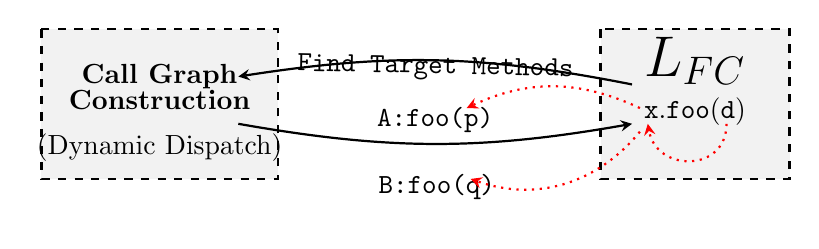
\begin{tikzpicture}
			\def\xc{3.5}
			\def\yc{0}
			\def\dist{2.8}
			\draw [draw=black, dashed, thick, fill=black!5] (-3.5 + \xc,0.7 + \yc,0) rectangle (-0.5 + \xc, -1.2 + \yc); % call graph construction
			\draw [draw=black, dashed, thick, fill=black!5] (0.8 + \xc + \dist,0.7 + \yc,0) rectangle (3.2 + \xc + \dist,-1.2 + \yc); % LFC
			\node (cg) at(-2 + \xc, 0.1 + \yc) {\bf Call Graph};
			\node (con) at (-2 + \xc, -0.2 + \yc) {\bf Construction};
			\node (vir) at (-2 + \xc, -0.8 + \yc) {(Dynamic Dispatch)};
			\node (l) at (2 + \xc + \dist, 0.3 + \yc) {\huge $\boldsymbol{L_{FC}}$};
			\node (c) at (2 + \xc + \dist, -0.35 + \yc) {$\mathtt{x.foo(d)}$};
			\node at (1.5 + \xc, -0.45 + \yc) {$\texttt{A:foo(p)}$};
			
			\path[-stealth]
			
			(1.2 + \xc + \dist, 0.0 + \yc) edge[sloped, thick, bend right=10] node[xshift=-0.0cm, yshift=-0.1cm]{\texttt{Find Target Methods}} (-1.0 + \xc, 0.1 + \yc) % find targets
			
			(-1.0 + \xc, -0.5 + \yc) edge [sloped, thick, bend right=10] node[xshift=0.02cm, yshift=-0.55cm]{$\texttt{B:foo(q)}$} (1.2 + \xc + \dist, -0.5 + \yc) % cg to x.foo

			(2.4 + \xc + \dist, -0.5 + \yc) edge[red, thick, dotted, in=-80, out=-90, loop, looseness=1.6, below] node[yshift=0.35cm]{{\Large \ScissorLeft}} (1.4 + \xc + \dist, -0.5 + \yc) % d to x
			
			(1.3 + \xc + \dist, -0.3 + \yc) edge[red, thick, dotted, sloped, bend right=25] node[yshift=-0.34cm]{{\Large \ScissorLeft}} (-0.9 + \xc + \dist, -0.3 + \yc) % x to p
			
			(1.3 + \xc + \dist, -0.6 + \yc) edge[red, thick, dotted, sloped, bend left=35] node[yshift=-0.34cm]{{\Large \ScissorLeft}} (-0.85 + \xc + \dist, -1.2 + \yc) % x to q
			;
			\end{tikzpicture}
		}
\vspace*{-3.5ex}
		\caption{Disconnection in the value flows between parameter passing in \manuLFC and
		dynamic dispatch at a virtual callsite.}
		\label{fig:MissingCGValueFlow}
\vspace*{-1.5ex}
	\end{figure}
\end{comment}

\subsubsection{\LFCR: Necessity, Challenges, and Our Solution}
\label{subsubsec:challenges}




\begin{comment}
Naturally, one may attempt to exploit Melski-Reps reduction \cite{melski2000interconvertibility} to obtain the new CFL-reachability formulation from their corresponding inclusion-based formulation. Unfortunately, the new CFL-reachability formulation does not have an equivalent set-constraint formulation as its form would be an intersection of several CFLs which has been proven to be undecidable \cite{reps2000undecidability}.
\end{comment}

\hl{Our primary contribution in this research is demonstrating the feasibility of incorporating on-the-fly callgraph construction into the specification of \kcs{k} using CFL-reachability.} In particular,
we introduce \LFCR (as the intersection of three CFLs)
as the first % complete 
CFL-reachability formulation of
\kcs{k} with built-in call graph construction, thereby overcoming the limitations of
\manuLFC (as the intersections of two CFLs) discussed above. It is worth emphasizing that
\LFCR operates on a new
PAG representation that is fundamentally different from the one operated on by \manuLFC. As the secondary contribution of this research, we demonstrate the utility of \LFCR
by introducing the first precision-preserving pre-analysis
for accelerating \kcs{k} with selective context-sensitivity. As discussed above, a recent \manuLFC-based
pre-analysis always loses precision.

\begin{comment}
We have designed \LFCR as the intersection of three CFLs to facilitate 
\LFCR-enabled CFL-reachability analyses. By noting that
\kcs{\infty} is undecidable and thus both the \manuLFC- and \LFCR-path
problems are undecidable (implying that either is a context-sensitive language
rather than a single CFL) \cite{reps2000undecidability}, 
\end{comment}

When developing \LFCR, we are required to reason about CFL reachability  to 
support parameter passing  prescribed by \kcs{k}. For
a virtual call $\texttt{r}.\texttt{m}(a_1, \dots, a_n)$ at callsite 
\textcolor{red}{c}, passing any of its
arguments $a$ to its corresponding
parameter $p$ of a   target method $m'$ that is yet to be discovered at this
callsite by \LFCR itself
under a given context $\CC$ must be done by establishing a CFL-reachability path in
a PAG representation of the program, starting from $a$, passing through the receiver variable $\texttt{r}$ to trigger dynamic dispatch, and
finally, ending at $p$, which is the corresponding parameter of $m'$ that is dispatched based on the
dynamic type of the object pointed by \texttt{r}
under the given context $\CC$. Relating $a$ to $\texttt{r}$   is non-trivial
if $a=a_i$ (for some $i$), i.e., $a\neq \texttt{r}$. In addition, in a CFL-reachability formulation, some
context elements in $\CC$ are usually consumed (i.e., balanced out according to \manuLC given in
\Cref{eqn:callsiteLC}) during the traversal for performing
 dynamic dispatch  and must thus be restored in order to enable \texttt{d} to be
passed to \texttt{p} under still the same given context \CC.
Below we list 
three challenges faced in handling this parameter passing task during the
on-the-fly call graph construction: 
 \begin{itemize}[leftmargin=*]
 \item  \challenge{1}.  How do we pass \texttt{r} to the  ``this'' variable of a target method invoked at callsite \textcolor{red}{c} 
 precisely (by avoiding
the precision loss illustrated with the code given in \Cref{fig:recvobj})?
 
  \item  \challenge{2}.  
  How do we establish a CFL-reachability path in a PAG representation of the program
  from   $a_i$ to $p_i$ passing through \texttt{r} in order to trigger
  dynamic dispatch during the course of parameter passing, where
  $p_i$ is the $i$-th parameter of a target method $m'$ discovered 
  at callsite \textcolor{red}{c} under  $\CC$?
 % passing for a set $T_{\scriptsize \LFCR}$ of    target methods discovered by \LFCR at callsite
 % \textcolor{red}{c}, such that $T_{\scriptsize \LFCR} \supseteq T_{\kcs{k}}$, where $T_{\kcs{k}}$ is  the set of target methods that are found by   \kcs{k} at callsite  \textcolor{red}{c} under context \textcolor{red}{c}?
 
 %or more specifically $\textcolor{red}{c} \mdoubleplus  \CC$, i.e., $[\textcolor{red}{c},c_1,...,c_n]$?  

 %\item {\bf CHL3.} Where do we perform dynamic dispatch for a virtual callsite during the
% CFL-reachability traversal for finding its receiver objects: at this callsite or the allocation sites where these receiver objects are created? 
 
 \item \challenge{3}. How
 do we ensure we can pass $a_i$ to $p_i$ for the target method $m'$ invoked 
at callsite \textcolor{red}{c}
 with a (correct) context abstraction that represents parameter passing
 for callsite \textcolor{red}{c}
  under $\CC$?
 
 %How do we ensure that parameter passing at a virtual callsite (with dynamic dispatch  performed by \LFCR itself) happens correctly with respect to \kcs{k} \cite{shivers1991control}?

%as in the demand-driven\manuLFC-based formulation \cite{sridharan2006refinement} (with dynamic dispatch being  performed by separate algorithm)?

 
 %\item {\bf CHL5.} 
 %How do we 
% ensure that the contexts
%just before and after parameter passing at a virtual callsite are identical when
%CFL-reachability-enabled
%dynamic dispatch happens in between?
 
 %How to ensure the context after dispatching are same as the traditional \manuLFC formulation that has an oracle for telling where to dispatch?   
  \end{itemize}

We  now give a high-level  overview of our solution  by using our motivating example 
(\Cref{fig:motivatingExample}). To support on-the-fly call graph construction
by itself,
\LFCR operates on a new PAG representation  shown in \Cref{fig:pag1}, which differs fundamentally from the PAG (\Cref{fig:pag2}) operated on by \manuLFC. In our formulation, we find that \texttt{v} points to \commentfont{O1} only due
to the existence of the following unique path from \commentfont{O1} to \texttt{v}, with the underlying technical details being explained
in \Cref{sec:CFL}:
{
\setlength{\abovedisplayskip}{4ex}
%\setlength{\belowdisplayskip}{1.5ex}
\begin{equation}
  \centering
\label{eq:ex-patho1-to-v}
\begin{tabular}{l} 
% \footnotesize
\vspace*{1ex}
\begin{tikzpicture}[-, remember picture,overlay]
%line
\def\lx{11.7}\def\ly{0.1}
\def\dy{-0.80}
\def\nx{-.4}\def\ny{-1.55}
\def\offset{0.25}
%rectangle height
\def\chIIaabove{0.5}\def\chIIabelow{0.5}
\def\chIIbabove{0.4}\def\chIIbbelow{0.5}
\def\chIIIaabove{0.5}\def\chIIIabelow{0.5}
\def\chIIIbabove{0.4}\def\chIIIbbelow{0.5}
\def\chIVaabove{0.6}\def\chIVabelow{0.6}
\def\chIVbabove{0.5}\def\chIVbbelow{0.6}
%rectangle location
\def\chIIastartx{\lx-4.55}
\def\chIIIastartx{\lx-2.86}
\def\chIIIaendx{\lx-.1}
\def\chIIIbstartx{\nx}
\def\chIIbstartx{\nx+6.15}
\def\chIIbendx{\nx+9.1}

\draw [draw=\chIVcolor, fill=\chIVcolor] (\chIIastartx-.1,\ly+\chIVaabove) rectangle (\chIIIaendx+.2,\ly-\chIVabelow); % CH4a-blue1
\draw [draw=\chIVcolor, fill=\chIVcolor] (\chIIIbstartx-.1,\ny+\chIVbabove) rectangle (\chIIbendx+.22,\ny-\chIVbbelow); % CH4b-blue2
\draw [draw=\chIIcolor, fill=\chIIcolor] (\chIIastartx,\ly+\chIIaabove) rectangle (\chIIIastartx,\ly-\chIIabelow); % CH2a-red1
\draw [draw=\chIIcolor, fill=\chIIcolor] (\chIIbstartx,\ny+\chIIbabove) rectangle (\chIIbendx+0.12,\ny-\chIIbbelow); % CH2b-red2
\draw [draw=\chIIIcolor, fill=\chIIIcolor] (\chIIIastartx,\ly+\chIIIaabove) rectangle (\chIIIaendx,\ly-\chIIIabelow); % CH3a-green1
\draw [draw=\chIIIcolor, fill=\chIIIcolor] (\chIIIbstartx+0.1,\ny+\chIIIbabove) rectangle (\chIIbstartx,\ny-\chIIIbbelow); % CH3b-green2


\draw(\lx-\offset, \ly) -- (\lx, \ly) -- (\lx, \dy);
\draw[dashed] (\lx, \dy) -- (\nx,\dy);
\draw(\nx,\dy) -- (\nx, \ny);
\draw[->] (\nx, \ny) -- (\nx+\offset, \ny);
\end{tikzpicture}
\commentfont{O1}$\xrightarrow{\new[\texttt{O}]}
\texttt{o1}\xrightarrow[\hat{\mathtt{c1}}]{\assign}
\texttt{o} \xrightarrow{\storefield{f}} \texttt{d}
\xrightarrow{\inewfield{\texttt{D}}}$ \commentfont{D1} 
$\xrightarrow{\new[\texttt{D}]} 
\texttt{d}$ $\xrightarrow[\hat{\boxed{\texttt{c3}}}]{\store[1]}\texttt{x}\xrightarrow[\check{\texttt{c1}}]{\iassign}\texttt{a} $ $\xrightarrow{\inewfield{\texttt{A}}}$\commentfont{A1} \\[6ex]
% \footnotesize 
$\xrightarrow{\new[\texttt{A}]}\texttt{a}\xrightarrow[\hat{\texttt{c1}}]{\assign}\texttt{x} \xrightarrow[\check{\boxed{\texttt{c3}}}]{\assign} \texttt{x\#c3}$ $\xrightarrow[\hat{\texttt{c3}}]{\indispatch[\texttt{A}]}\texttt{this}^\texttt{A:foo()}
\xrightarrow{\load[1]}\texttt{p}
    \xrightarrow{\load[\texttt{f}]} \texttt{v}$ \\[3ex]
% \begin{tikzpicture}[-, remember picture,overlay]
% \def\lx{7.1}\def\ly{.95}
% \def\dy{.45}\def\ny{.068}
% \draw(\lx, \ly) -- (\lx+.1, \ly) -- (\lx+.1, \dy);
% \draw[dashed] (\lx+.1, \dy) -- (-.12,\dy);
% \draw(-.12,\dy) -- (-.12, \ny);
% \draw[->] (-.12, \ny) -- (0.06, \ny);
% \end{tikzpicture}
% \footnotesize 
% $\xrightarrow[\hat{\texttt{c3}}]{\indispatch[\texttt{A}]}\texttt{this}^\texttt{A:foo()}
% \xrightarrow{\load[1]}\texttt{p}
%     \xrightarrow{\load[\texttt{f}]} \texttt{v}$
\end{tabular}
\end{equation}
}

This path represents the flow of \commentfont{O1} to \texttt{v} by passing a sequence of
two calls,  ``\inline{bar(a,o1); // c1}'' and ``\inline{x.foo(d); // c3}''. Consider the
parameter passing for \texttt{d} under  context $\CC=[\texttt{c1}]$ at ``\inline{x.foo(d); // c3}'', which has only one target \texttt{A:foo()}.
 Instead of passing \texttt{d} to \texttt{p} directly via  one inter-procedural
\assign edge 
$d\xrightarrow[\hat{{\mathtt{c3}}}]{\assign} \mathtt{p}$
as in \manuLFC (\Cref{eq:LFCPathCGPreciseI}), which is illustrated in
\Cref{fig:pag2}, since \manuLFC requires  \texttt{A:foo()}
 to be found separately outside \manuLFC, \LFCR passes \texttt{d} to \texttt{p} indirectly
 via a sequence of PAG edges, along the path given in
 \Cref{eq:ex-patho1-to-v} (shown also in  \Cref{fig:pag1}),  by discovering this dispatch target dynamically during
 the sub-path from \texttt{d} to \texttt{p}. Briefly, we address 
 \challenge{1} by requiring $\new[\texttt{A}]$ to be matched with $\indispatch[\texttt{A}]$.
 We address \challenge{2} by first storing \texttt{d} into a special field of \texttt{x}
 to trigger dynamic dispatch at this callsite 
 and then loading it from the same special field of $\texttt{this}^\texttt{A:foo()}$
 into \texttt{p} later (with the two sub-paths highlighted in
 \crule[\chIIcolor]{1.5ex}{1.5ex}). In addition, we
 perform dynamic dispatch correctly at this callsite under 
 $\CC=[\texttt{c1}]$ (with the sub-path highlighted in \crule[\chIIIcolor]{1.5ex}{1.5ex}) as
 in the case of \manuLFC. We address \challenge{3} by passing \texttt{d} to \texttt{p}
 also correctly under  [\texttt{c3},\texttt{c1}], where \texttt{c3}  records the  callsite as in
 \manuLFC (\Cref{eq:LFCPathCGPreciseI}) for which parameter passing takes place
 and \texttt{c1} signifies further the
 context under which the receiver object \commentfont{A1} flows into the receiver
 variable \texttt{x} at this callsite
  (with the sub-path highlighted in \crule[\chIVcolor]{1.5ex}{1.5ex}). The significance
  of the two below-edge labels,
  $\hat{\boxed{\texttt{c3}}}$ and $\check{\boxed{\texttt{c3}}}$, in addressing \challenge{3} cannot be
  over-emphasized. This ensures that if we start dynamic dispatch at callsite 
  \texttt{c3} under context $\CC=[\texttt{c1}]$, we will always return
  to the same callsite    under the same context 
  even though  $\texttt{c1}$ is lost (i.e., balanced out due to
  $\hat{{\texttt{c1}}}\check{{\texttt{c1}}}$) just after
  $\mathtt{x}\xrightarrow[\check{{\mathtt{c1}}}]{\iassign} \mathtt{a}$ at the beginning of the
  traversal for performing
  dynamic dispatch at callsite \texttt{c3}.
  To address  \challenge{1} -- \challenge{3}, we
  have designed \LFCR to be the intersection of three CFLs operating on a new
  PAG representation as described below.